%%%%%%%%%%%%%%%%%%%%%%%%%%%%%%%%%%%%%%%%%%%%%%
%%%%%%%%%%%%%%%%%%%%%%%%%%%%%%%%%%%%%%%%%%%%%%
%%%%%%%%%%%%%%%%%%%%%%%%%%%%%%%%%%%%%%%%%%%%%%
\chapter{Results for Thermalisation}
\label{appendix:thermalisation_results}
%%%%%%%%%%%%%%%%%%%%%%%%%%%%%%%%%%%%%%%%%%%%%%
%%%%%%%%%%%%%%%%%%%%%%%%%%%%%%%%%%%%%%%%%%%%%%
%%%%%%%%%%%%%%%%%%%%%%%%%%%%%%%%%%%%%%%%%%%%%%


%%%%%%%%%%%%%%%%%%%%%%%%%%%%%%%%%%%%%%%%%%
\section{Thermalisation in the Pauli Blocked Regime}
\label{app:sec:pauliblockingle}
%%%%%%%%%%%%%%%%%%%%%%%%%%%%%%%%%%%%%%%%%%
In this section, we derive the analytic approximations for the thermalisation times in the low energy, zero temperature approximations, first for $m_\chi\lesssim \mcrit$.

The average energy lost in an interaction can be calculated as
\begin{equation}
    \langle \Delta K_\chi \rangle = \frac{1}{\Gamma^-}\int_0^{\qomax} dq_0\; q_0 \frac{d \Gamma^-}{d q_0},
    \label{app:eq:avg_energy_loss}
\end{equation}
where the differential interaction rates are the $q_0$ integrands of Eq.~\ref{app:eq:gamma_low_2}. Evaluating Eq.~\ref{app:eq:avg_energy_loss} for matrix elements $\Msq = \alpha t^n$ yields
\begin{align}
    \langle \Delta K_\chi^{ (n = 0)} \rangle & = \frac{4}{7}K_\chi,\\
    \langle \Delta K_\chi^{ (n = 1)} \rangle & = \frac{5}{9}K_\chi,\\
    \langle \Delta K_\chi^{ (n = 2)} \rangle & = \frac{28}{55}K_\chi.
\end{align}

We follow Ref.~\cite{Bertoni:2013bsa_dec_DarkMatterThermalization} and define the thermalisation time as the sum of the average time between interactions, 
\begin{equation}
    \tth = \sum_{n=0}^{N_2} \frac{1}{\Gamma^-(K_{n})} \sim \sum_{n=N_1}^{N_2} \frac{1}{\Gamma^-(K_{\chi, n})},
    \label{app:eq:therm_time_defn}
\end{equation}
where $K_{n}$ is the DM kinetic energy after $n$ collisions. 
This process has two stages: one in which the interactions are unaffected by Pauli blocking, which takes $N_1$ collisions, and the next $N_2$ collisions in which Pauli blocking is in effect. 

The DM will reach thermal equilibrium with the targets when $K_\chi \leq \Teq$, the equilibrium temperature of the star. 
If Pauli blocking affects any part of the thermalisation process, then $K_{N_1 + N_2}$ is related to the kinetic energy after the initial $N_1$ interactions, $K_{N_1}$ though
\begin{equation}
    K_{N_1 + N_2} = K_{N_1}\left( 1 - \frac{\langle \Delta K_\chi \rangle}{K_{\chi}}\right)^n = \Teq,
    \label{app:eq:Kchi_Teq_rel}
\end{equation}
where we have used the fact that the fractional energy loss in the PB regime is independent of $K_\chi$.

As shown in Appendix~\ref{app:sec:int_low_temp}, the interaction rates for matrix elements $\Msq = \alpha t^n$, are of the form $\Gamma^-\propto (K_\chi)^{n+2}$. Substituting this into Eq.~\ref{app:eq:therm_time_defn} and using Eq.~\ref{app:eq:Kchi_Teq_rel} yields
\begin{align}
    \tth & \propto \sum_{i=N_1}^{N_2} (K_{i})^{-(n+2)}\\
    & = \frac{1}{K_{N_1}^{n+2}}\sum_{i=N_1}^{N_2}\left(\left( 1 - \frac{\langle \Delta K_\chi \rangle}{K_{\chi}}\right)^{-(n+2)}\right)^i\\
    & = \frac{1}{K_{N_1}^{n+2}}\frac{\left(1 - \frac{\langle \Delta K_\chi \rangle}{K_{\chi}}\right)^{(n+2)(1-N_1)} - \left(1 -\frac{\langle \Delta K_\chi \rangle}{K_{\chi}}\right)^{-(n+2) N_2}}{-1 + \left(1 - \frac{\langle \Delta K_\chi \rangle}{K_{\chi}}\right)^{n+2}}\\
    & \sim  \frac{1}{K_{N_1}^{n+2}} \frac{\left(1 - \frac{\langle \Delta K_\chi \rangle}{K_{\chi}}\right)^{-(n+2) N_2}}{1 - \left(1 - \frac{\langle \Delta K_\chi \rangle}{K_{\chi}}\right)^{n+2}}\quad \text{for}\quad N_2 > N_1\\
    & =  \frac{1}{K_{N_1}^{n+2}} \left( \frac{T_{eq}}{K_{N_1}}\right)^{-(n+2)}\frac{1}{1 - \left(1 - \frac{\langle \Delta K_\chi \rangle}{K_{\chi}}\right)^{n+2}}\\
  \implies \tth  & \propto \frac{1}{\Teq^{n+2}}\frac{1}{1 - \left(1 - \frac{\langle \Delta K_\chi \rangle}{K_{\chi}}\right)^{n+2}}.
\end{align}

The resulting thermalisation times for $n = 0, 1, 2$ in terms of the DM-target scattering cross-section $\sigma_{i\chi}$ are
\begin{align}
    \tthn{0} & = \frac{147}{16}\frac{\pi^2 m_\chi}{(\mi + \mchi)^2} \frac{1}{\sigmaichin{0}} \frac{1}{\Teq^2},\\
    \tthn{1} & = \frac{2187}{304}\frac{\pi^2 m_\chi^2 \mi^2}{(\mi + \mchi)^2(\mi^2 + \mchi^2)} \frac{1}{\sigmaichin{1}} \frac{1}{\Teq^3}\frac{1 - B(\Rstar)}{B(\Rstar)},\\
    \tthn{2} & = \frac{27451875}{4925248}\frac{\pi^2 m_\chi^3\mi^4}{(\mi + \mchi)^2(\mi^2 + \mchi^2)^2} \frac{1}{\sigmaichin{2}} \frac{1}{\Teq^4}\left[\frac{1 - B(\Rstar)}{B(\Rstar)}\right]^2.
\end{align}




%%%%%%%%%%%%%%%%%%%%%%%%%%%%%%%%%%%%%%%%%%%%%%%%%%%%%%%%%%%%%%%%%%%%%%%%%%%%%%%%%%%%
%%%%%%%%%%%%%%%%%%%%%%%%%%%%%%%%%%%%%%%%%%%%%%%%%%%%%%%%%%%%%%%%%%%%%%%%%%%%%%%%%%%%
\section{Thermalisation of super-heavy DM}
\label{app:sec:thermsuperheavy}
%%%%%%%%%%%%%%%%%%%%%%%%%%%%%%%%%%%%%%%%%%%%%%%%%%%%%%%%%%%%%%%%%%%%%%%%%%%%%%%%%%%%
%%%%%%%%%%%%%%%%%%%%%%%%%%%%%%%%%%%%%%%%%%%%%%%%%%%%%%%%%%%%%%%%%%%%%%%%%%%%%%%%%%%%



For DM that is heavier than the critical mass  $m_\chi\gtrsim m_\chi^{\rm crit}$,
the energy lost in each scatter is a tiny fraction of the total DM kinetic energy. Moreover, the average time between collisions is typically on the order of fractions of a second. This warrants the use of a continuous approximation in this regime rather than performing the discrete summation. The thermalisation time is then found by integrating the rate at which the DM kinetic energy changes, 
\begin{equation}
    \frac{dK_\chi}{dt} = -\Gamma^{-}(K_\chi) \langle\Delta K_\chi\rangle,  
    \label{app:eq:contttherm}
\end{equation}
from the initial kinetic energy, $K_\chi=m_\chi\left(\frac{1}{\sqrt{B(r)}}-1\right)$, to the final value $T_{\rm eq}\ll m_\chi$. For a constant cross-section ($n=0$), we substitute  Eqs.~\ref{app:eq:intraten0largem} and \ref{ch6:eq:aveElossn0largem} into the expression above leading to
\begin{equation}
    \tthn{0} \sim \frac{9 \pi^2 m_\chi}{8 (\mbeff)^2 \kinFi^2 \sigma_{i\chi}^{n=0}}\log\left[\frac{m_\chi}{T_{\rm eq}}\left(\frac{1}{\sqrt{B(\Rstar)}}-1\right)\right].
    \label{app:eq:tthemheavy0}
\end{equation}
Taking the final temperature to be $T_{\rm eq}=10^3\K$ and $B(\Rstar)=0.5$, this yields 
\begin{equation}
    \tthn{0} \sim 1.7  \yrs \left(\frac{m_\chi }{10^{10}\GeV}(r)\right)\left(\frac{0.5\;m_n}{\mbeff(0)}\right)^{2}\left(\frac{0.2\GeV}{\kinFi(0)}\right)^{2}\left(\frac{10^{-45}\cm^2}{\sigma_{i\chi}^{n=0}}\right).    
\end{equation}
%
Repeating for $d\sigma\propto t^n$ ($n=1,2$), we calculate the thermalisation time for $n=1$ to be
\begin{eqnarray}
    \tthn{1} &\sim& \frac{9\pi^2 m_\chi}{ 64 \mbeff \kinFi^3 \sigma_{i\chi}^{n=1}}\left[\frac{1-B(\Rstar)}{B(\Rstar)}\right] \log\left[\frac{m_\chi}{T_{\rm eq}} \left(\frac{1}{\sqrt{B(\Rstar)}}-1\right)\right],\\
    &\sim& 3.5 \yrs\; \left(\frac{m_\chi}{10^{10} \GeV}\right)\left(\frac{0.5\;m_n}{\mbeff(0)}\right) \left(\frac{0.2\GeV}{\kinFi(0)}\right)^{3}\left(\frac{10^{-45}\cm^2}{\sigma_{i\chi}^{n=1}}\right),
\end{eqnarray}
and that for $n=2$ to be
\begin{eqnarray}
    \tthn{2} &\sim& \frac{5 \pi^2 m_\chi}{ 32 \kinFi^4\sigma_{i\chi}^{n=2}} \left[\frac{1-B(\Rstar)}{B(\Rstar)}\right]^2 \log\left[\frac{m_\chi}{T_{\rm eq}}\left(\frac{1}{\sqrt{B(\Rstar)}}-1\right)\right],\\
    &\sim& 3.5 \yrs \left( \frac{m_\chi}{10^{10} \GeV}\right) \left(\frac{0.2\GeV}{\kinFi(0)}\right)^{4}\left(\frac{10^{-45}\cm^2}{\sigma_{i\chi}^{n=2}}\right). 
\end{eqnarray}







%%%%%%%%%%%%%%%%%%%%%%%%%%%%%%%%%%%%
\section[Thermalisation time for {\it s}- and {\it t}-dependent interactions]{Thermalisation time for $s$- and $t$-dependent interactions}
\label{app:sec:sdeptherm}
%%%%%%%%%%%%%%%%%%%%%%%%%%%%%%%%%%%%


In Section~\ref{ch6:sec:thermstandard}, we assumed $\Msq\propto t^n$ when deriving analytical approximations for the thermalisation timescale. To understand the behaviour of the thermalisation time for the operators in Table.~\ref{ch1:tab:opers_defn_full}, we can make use of the results for $t^n$ dependent interactions. For cross-sections that are linear combinations of different powers of $t$, we can approximate the thermalisation time using the previous results in the following way
\begin{eqnarray}
\Msq &=& a_0 + a_1 t + a_2 t^2,\\
\sigma &=& a_0\sigma_0 + a_1 \sigma_1 + a_2 \sigma_2,\\
\frac{1}{\tth} &\sim& \frac{a_0}{ \tthn{0}(\sigma_{i\chi}=\sigma_0)} + \frac{a_1} {\tthn{1}(\sigma_{i\chi}=\sigma_1)} 
 + \frac{a_2}{  \tthn{2}(\sigma_{i\chi}=\sigma_2)}. 
\label{app:eq:ttherm_weighted}
\end{eqnarray}
Hence, the inverse of the thermalisation time will be given by a weighted linear combination of the inverse times for each contribution. As higher powers of $t$ require significantly longer thermalisation times, for coefficients of similar size, the resulting sum will be dominated by the lowest power of $t$ appearing in  $\Msq$.  We can thus identify the dominant terms for operators D1-D4  based on power counting, which we have listed in Table~\ref{ch1:tab:opers_defn_full}.

 For $s$-dependent amplitudes, we can, in principle, use the interaction rates calculated in Appendix~\ref{app:sec:capratesimple}, perform a series expansion in $K_\chi$  and repeat the same procedure outlined in Section~\ref{ch6:sec:thermstandard} for $s$-independent matrix elements. Interestingly, we find that for the purpose of calculating the thermalisation time, there is an easier way to obtain the correct result. One can indeed check that, at zero order in $\kinFi/\mbeff$, the resulting time for $s^1, s^2$ is equivalent to the constant case, with the matrix element calculated by setting 
\begin{equation}
    s\rightarrow (m_\chi+\mbeff)^2,
    \label{app:eq:ssubst}
\end{equation}
while the $s t $ case has a result equivalent to the $t$ case, with the matrix element calculated using the same substitution. This is, in practice, equivalent to setting both the DM and neutron targets at rest. There is, however, an important exception when it comes to calculating the thermalisation time of a linear combination of these terms. In particular, when the amplitudes at order $\mathcal{O}(t^0)$, are proportional to combinations of $1,s,s^2$ such as
\begin{gather}
s-(m_\chi+\mbeff)^2,\nonumber\\
\left[s-(m_\chi+\mbeff)^2\right]^2,\nonumber\\
\left[s-(\mbeff)^2-m_\chi^2\right]^2-4(\mbeff)^2 m_\chi^2.\label{app:eq:m2veldep}
\end{gather}
All these combinations give a null result after applying substitution Eq.~\ref{app:eq:ssubst}. In such a case, one may think that the dominant term is given by some remaining $t^n$ term. It is worth noting that the expressions in  Eq.~\ref{app:eq:m2veldep}  appear in operators that, at low energy, are known as velocity-dependent because their matrix elements are proportional to positive even powers of the DM-target relative speed. Consequently, it is important not to neglect the motion of the targets in the neutron star, moving at relativistic speeds that are of the order of the Fermi velocity $v_F^2=2\kinFi/\mbeff$. In those cases, one should instead set $s$ to\footnote{We assume that $\mu\gg \mbeff/m_\chi^{\rm crit}$ when making this substitution.}
\begin{equation}
    s\rightarrow (m_\chi+\mbeff)^2+2m_\chi\kinFi.
    \label{app:eq:ssubstmu}
\end{equation}


In summary, operators D5, D8, and D9 can be safely expanded using Eq.~\ref{app:eq:ssubst}, while operators D6, D7, and D10 have velocity-dependent amplitudes and require Eq.~\ref{app:eq:ssubstmu}. 
The dominant terms for each operator can be found in Table~\ref{ch1:tab:opers_defn_full}. 
For equal values of the leading term in $\Msq$, the thermalisation time for each operator will be the same as the relevant $t^n$ power law. 


%%%%%%%%%%%%%%%%%%%%%%%%%%%%%%%%%%%%%%%%%%%%%%%%%%%%%%%%%%%%%%%
\section{Temperature distribution of captured dark matter}
\label{app:sec:minTempDerivation}
%%%%%%%%%%%%%%%%%%%%%%%%%%%%%%%%%%%%%%%%%%%%%%%%%%%%%%%%%%%%%%



As seen in Fig.~\ref{ch6:fig:thermtime}, interactions that depend on the momentum transfer, namely $d\sigma \propto t^n$ with $n = 1,2$, there are regions of the DM mass parameter space where thermalisation does not occur within the age of the star. For the DM masses and NS temperatures of interest, this region of non-thermalisation always occurs in the $m_\chi\ll \mcrit$ regime.
From Eqs.~\ref{ch6:eq:thermtimen0}, \ref{ch6:eq:thermtimen1} and \ref{ch6:eq:thermtimen2},  we can estimate the time required for the DM to reach a kinetic energy $K_\chi$ 
\begin{equation}
    t_{K_\chi} \propto \frac{1}{K_\chi^{n+2}}.
\end{equation}
% 
If the DM does not thermalise within the age of the star, it will instead reach a minimum temperature, $K_\chi^{\mathrm{min}}$.  Comparing the time required to achieve this temperature to the thermalisation time, $\tth$, i.e. to have reached the equilibrium temperature $\Teq$, we find 
\begin{equation}
    \frac{t_{K_\chi^\mathrm{min}}}{\tth}  \sim \left( \frac{\Teq}{K^{\rm min}_\chi} \right)^{n+2}. 
\end{equation}
Accounting for the case where the DM reaches thermalisation, we can write $K_\chi^\mathrm{min}$
\begin{align}
    K^{\rm min}_\chi & \sim \Teq \left(\max\left[ 1,\frac{\tth}{t_{K_\chi^\mathrm{min}}}\right]\right)^{\frac{1}{n + 2}}\\
           & \approx \Teq \left( 1 + \frac{\tth}{t_{K_\chi^\mathrm{min}}}\right)^{\frac{1}{n + 2}}. 
\end{align}
The population of captured DM will have a distribution of energies at any given time, with this distribution being peaked at this minimum energy.
As the orbital periods of the DM will be much shorter than the average time between interactions, the DM will be able to virialize between each interaction. Therefore, we can treat the DM as being contained within an isothermal sphere with temperature $K^{\rm min}_\chi > \Teq$. 

Finally, it is worth noting that at times  $t>\tth$, even though the thermalisation condition has been reached, the captured DM would consist of two components: a fraction of it (whose amount depends on time) would be in thermal equilibrium with the NS at temperature $T_{\rm eq}$; and another component still in the cooling down process. Assuming a  capture rate constant over time, the fraction of thermalised DM is 
\begin{equation}
    f_{\rm therm}(t) = \frac{t-t_{\rm therm}}{t}.
\end{equation}




%%%%%%%%%%%%%%%%%%%%%%%%%%%%%%%%%%%%%%%%%%%%%%%%%%%%%%%%%%%%%%%
\section[Quark-level vs hadron-level annihilation cross-sections]{Quark-level vs hadron-level annihilation\\cross-sections}
\label{sec:quarkhadron}
%%%%%%%%%%%%%%%%%%%%%%%%%%%%%%%%%%%%%%%%%%%%%%%%%%%%%%%%%%%%%%%

The annihilation cross-sections shown in Table~\ref{ch6:tab:annCS} are for DM annihilation to quark final states.  More properly, we should consider the hadron-level annihilation cross-section.
However, we are primarily concerned with the capture-annihilation equilibrium timescale and not the details of the annihilation process. Therefore, if the annihilation rate to hadrons is not significantly different from the quark-level result, this subtlety can be avoided. 

To check the validity of the quark-level approximation, we estimate the annihilation rate to hadrons, working at the lowest order in Chiral Perturbation Theory. We use couplings to the meson octet obtained from  ref.~\cite{Kumar:2018heq_dec_IndirectDetectionSubGeV}; for annihilation to baryons, the operators listed in Table~\ref{ch1:tab:opers_defn_full} are used. 
For DM masses in the range $m_\pi < m_\chi \lesssim m_{\rm charm} = 1.27\GeV$, we find that the cross-section for annihilation to hadrons differs by less than an order of magnitude than that for annihilation to quarks. For larger DM mass, the difference is negligible. Therefore, to simplify the discussion, we consider DM annihilation to quark final states for DM masses above the pion mass.


Below the pion mass, the only kinematically allowed DM annihilation channels would be to leptons or photons. The size of the DM couplings to these states would, in general, be unrelated to the DM-quark couplings we have assumed. (They are expected to be non-zero because they would be induced at loop level~\cite{Bell:2019pyc_jun_CaptureLeptophilicDark}, even if absent at tree level.)
However, due to the considerable Fermi energies of the electrons and muons near the centre of the NS, these channels will be Pauli blocked for the whole DM mass range below $m_\pi$, forbidding these annihilations from occurring. To remain as model-independent as possible, we will not consider lepton and photon annihilation channels.

Figure~\ref{app:fig:ann_xs_plots} shows $t_{\rm eq}$ contour lines in the $\Lambda_q-m_\chi$ plane for the NS benchmark model QMC-2, $\Tstareq=1000\K$ and two representative operators D7 (left) and D8 (right). 
Operators whose thermally averaged annihilation cross-section $\sigmav$ has a  $m_q/m_\chi$ leading order term, namely D1-D4 and D8 (see Table~\ref{ch6:tab:annCS}), exhibit a sudden change in the slope wherever a new annihilation channel opens (see dotted lines on the right panel of Fig.~\ref{app:fig:ann_xs_plots}). Note that the higher the cutoff scale $\Lambda_q$, the lower the scattering and annihilation cross-sections, resulting in a larger $t_{\rm eq}$ timescale. For lower $\Teq$ temperatures, DM requires more time to reach both equilibrium conditions, thermalisation and capture-annihilation. The variation of these results with respect to the NS configuration amounts at most to a factor of $\sim2$ in the $t_{\rm eq}$ contours (see shaded regions in the left panels) from the lightest configuration (QMC-1, $1\Msun$) to the heaviest (QMC-3, $1.9\Msun$) for most operators, with the sole exception of D4 for which this factor rises up to $\sim 2.4$. 

%%%%%%%%%%%%%%%%%%%%%%%%%%%%%%
\begin{figure*}
    \centering
    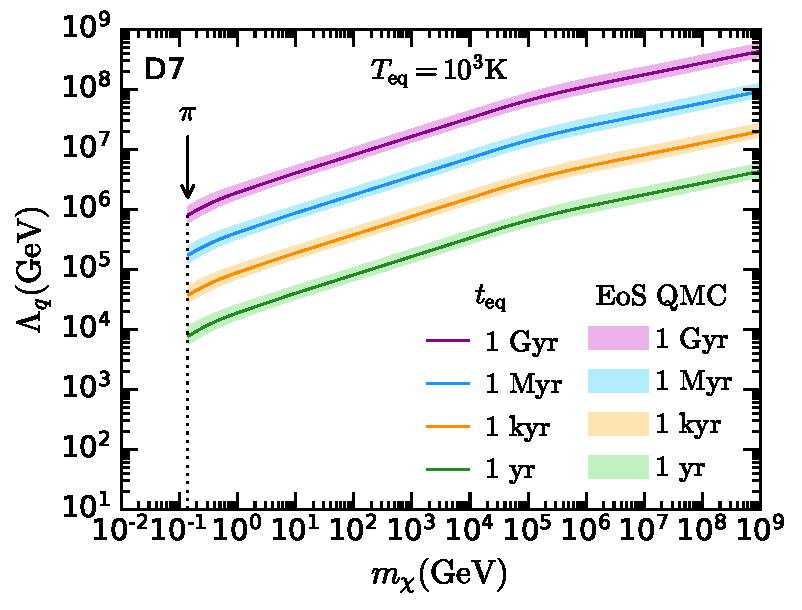
\includegraphics[width = 0.496\textwidth]{img/thermalisation/D7_Lambda_mdm_teq.pdf}
    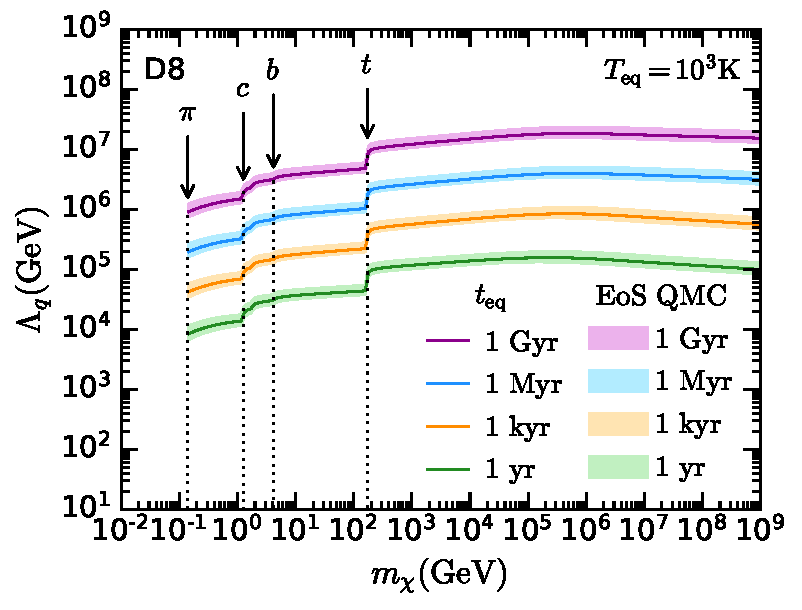
\includegraphics[width = 0.496\textwidth]{img/thermalisation/D8_Lambda_mdm_teq.pdf}    
    \caption[Contours of the capture annihilation timescale, $t_{\rm eq}$,  in the $\Lambda_q-m_\chi$ plane for operators D7 (left) and D8 (right) and $\Tstareq=1000\K$. ]{
    Contours of the capture annihilation timescale, $t_{\rm eq}$,  in the $\Lambda_q-m_\chi$ plane for operators D7 (left) and D8 (right) and $\Tstareq=1000\K$. 
    Solid lines represent the calculation for the NS benchmark model QMC-2, and shaded regions denote the variation with the NS choice for the QMC EoS family. 
    Dotted lines in the right panel indicate the mass thresholds for various annihilation channels.  
    }
    \label{app:fig:ann_xs_plots}
\end{figure*}
%%%%%%%%%%%%%%%%%%%%%%%%%%%%%%%%%%%%%%


%%%%%%%%%%%%%%%%%%%%%%%%%%%%%%%%%%%%%%%%%%%%%%%%%%%%%%%%%%%%%%%
\section[Capture-annihilation equilibrium for EFT operators]{Capture-annihilation equilibrium for\\EFT operators}
\label{app:sec:resultsEFTop}
%%%%%%%%%%%%%%%%%%%%%%%%%%%%%%%%%%%%%%%%%%%%%%%%%%%%%%%%%%%%%%%

\begin{figure*}
    \centering
    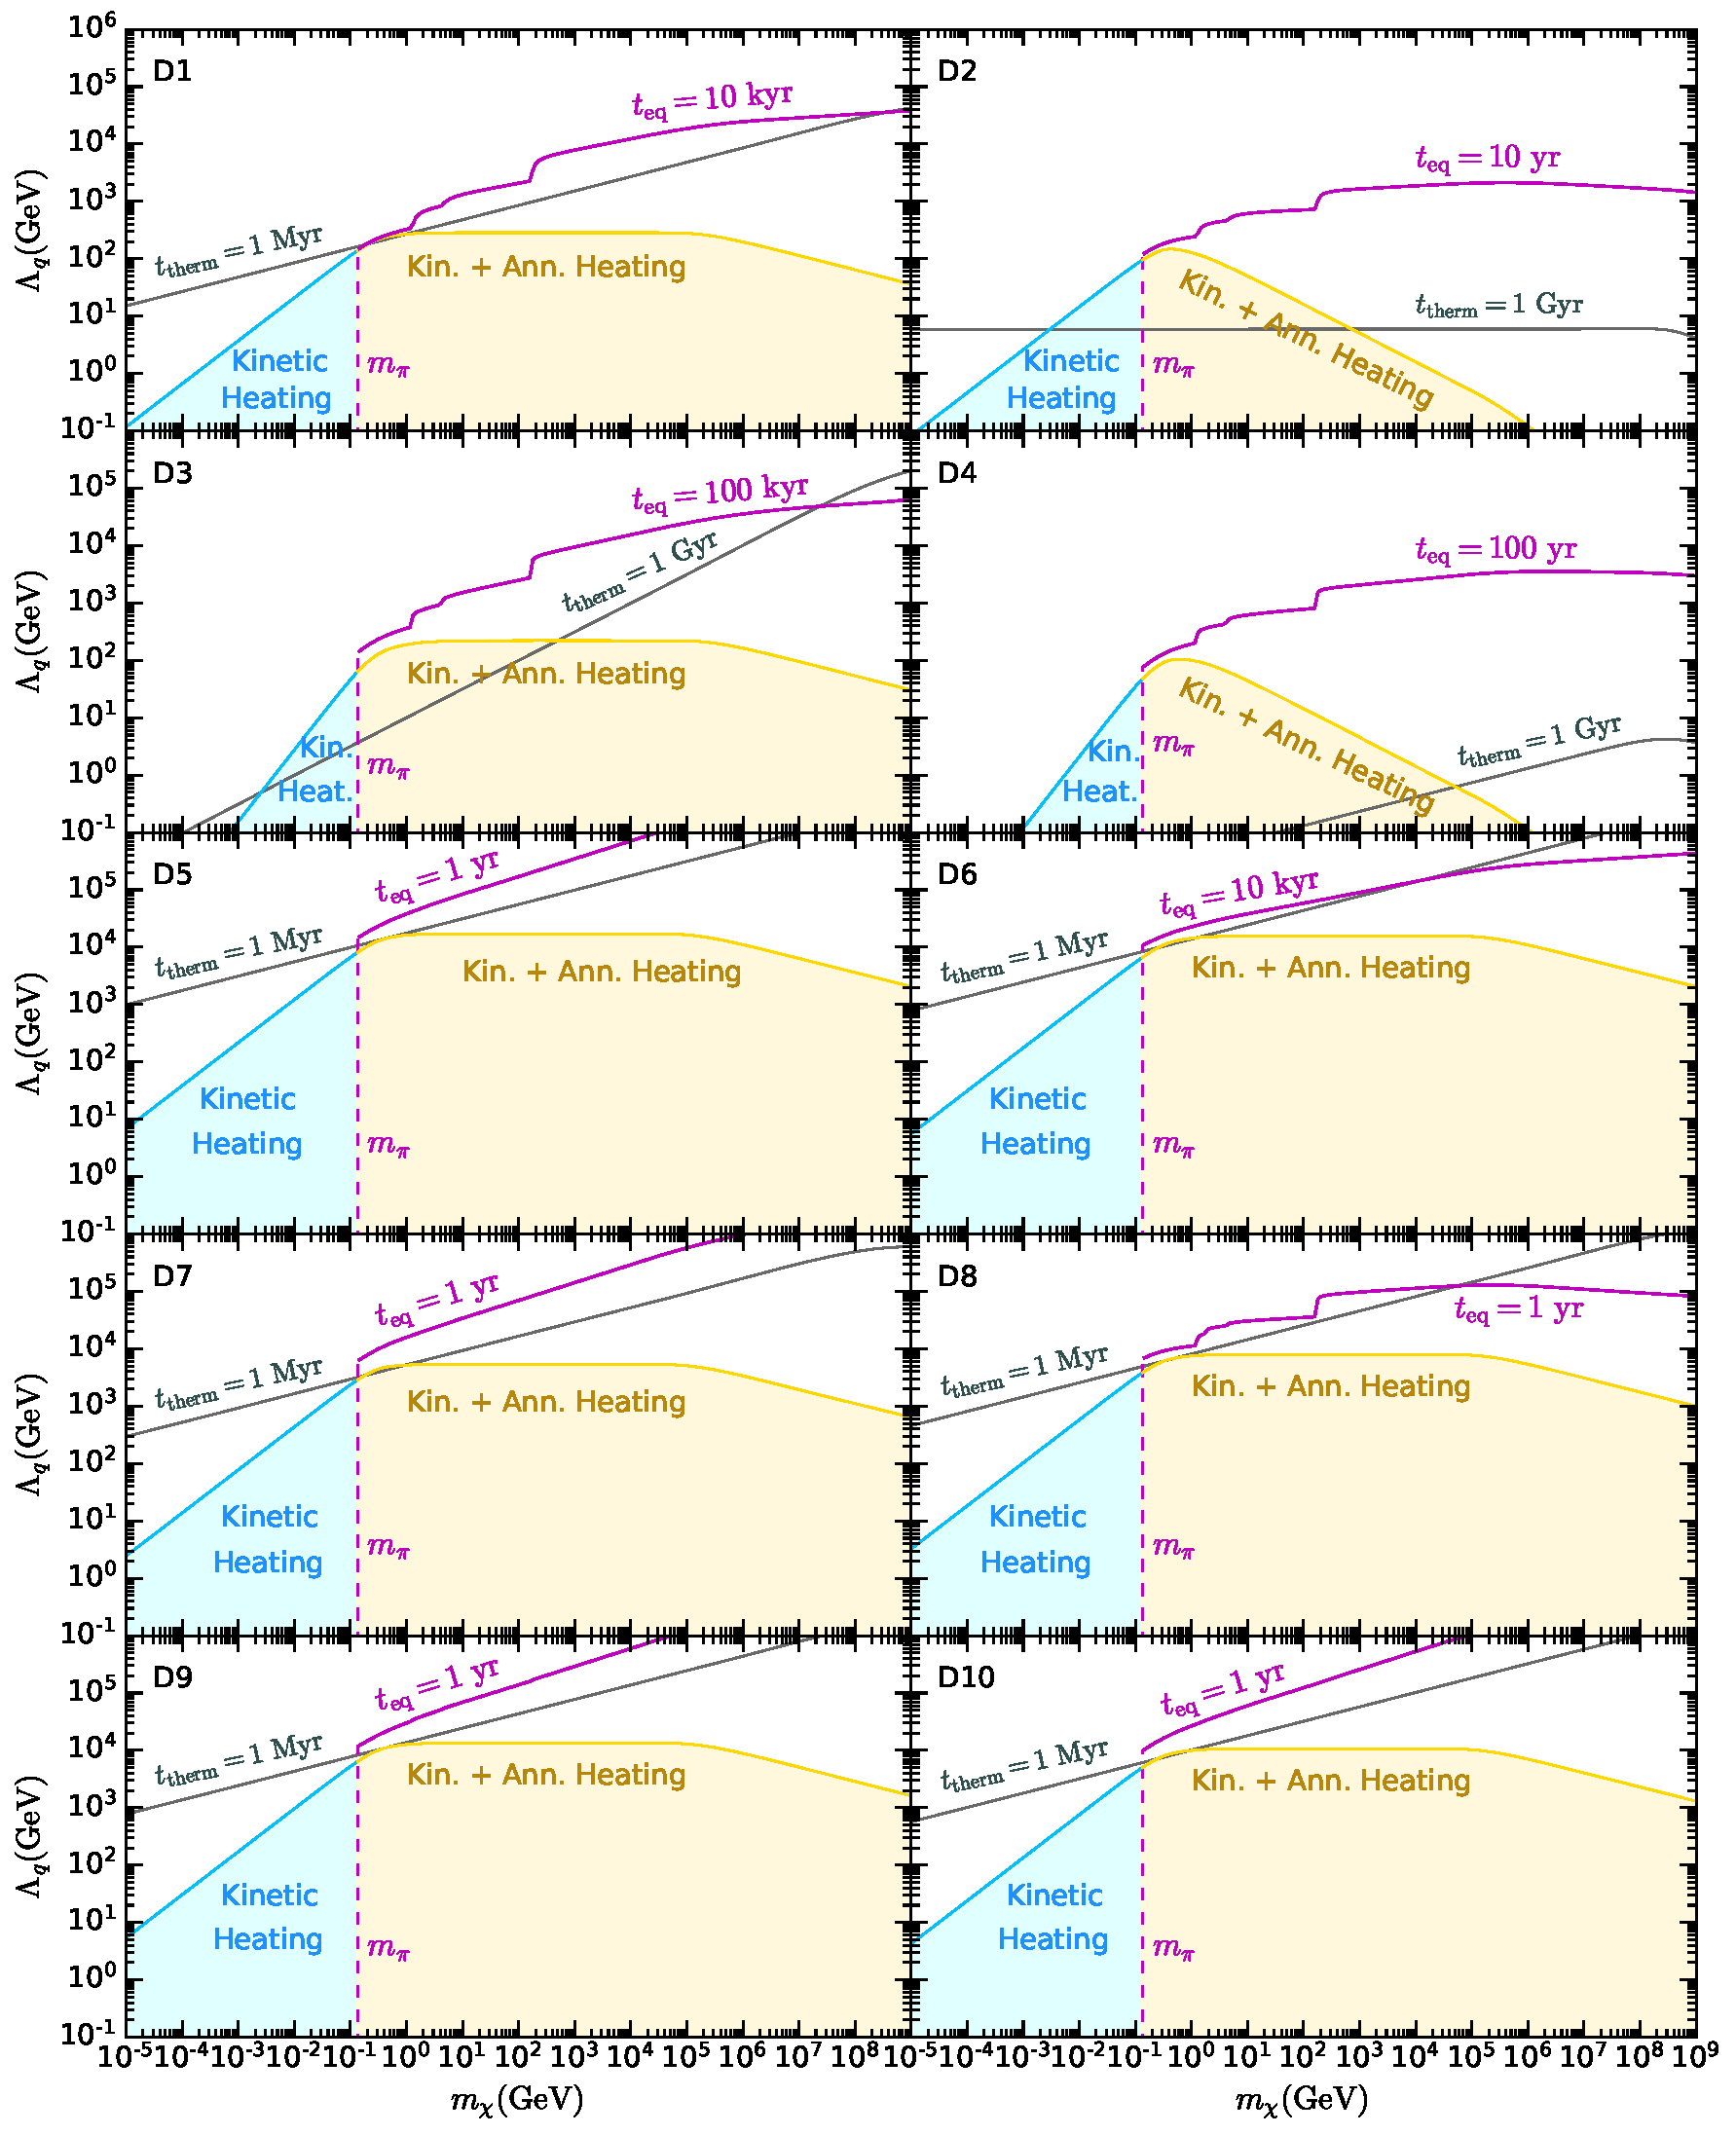
\includegraphics[width=\textwidth]{img/thermalisation/ann_heat_sensitivity.pdf}    
    \caption[Projected NS heating sensitivity for maximal capture efficiency, for the full set of DM-baryon interactions described by the EFT operators of Table~\ref{ch1:tab:opers_defn_full}.]{Projected NS heating sensitivity for maximal capture efficiency, for the full set of DM-baryon interactions described by the EFT operators of Table~\ref{ch1:tab:opers_defn_full}. We have used the QMC-2 ($1.5\Msun$) benchmark NS configuration.  
    Color coding as in Fig.~\ref{ch6:fig:NS_heating}. 
    }
    \label{app:fig:NS_heating2}
\end{figure*}



In Fig.~\ref{app:fig:NS_heating2}, we show isocontours of maximal capture (yellow and light blue lines) and capture-annihilation equilibrium (magenta lines) timescale in the $\Lambda_q-m_\chi$ plane for all  EFT operators.  
Values of $\Lambda_q$ below the $t_{\rm eq}$ lines result in smaller capture-annihilation equilibrium timescales. 
We can see in Fig.~\ref{ch6:fig:NS_heating} that for all operators, the $t_{\rm eq}$ timescale is always smaller than the time required for captured DM to thermalise. Captured DM achieves the steady state condition in a timescale as short as $\sim1\yr$ (D1, D6-D10) or as long as $10^5\yr$ (D3). 
Note that the displayed values of $t_{\rm eq}$ are the values for which the entire parameter space relevant for capture reaches equilibrium with annihilation. 

For D1 and D6-D10, we observe that captured DM achieves thermal equilibrium in less than $\sim 1\Myr$ (grey lines). 
On the other hand, as expected from Fig.~\ref{ch6:fig:thermtime} captured DM whose interactions are momentum suppressed, namely operators D2-D4, would never thermalise to the temperature expected from DM induced heating in $1\Gyr$, or even in less than the age of the 
Universe,
with the sole exception of the corner region of very light DM $m_\chi\lesssim 2\MeV$ and an even narrower corner of the parameter space for D4. 

Therefore, for all EFT operators,  the energy released in the annihilation process adds up to the energy deposited via capture, increasing the DM-induced heating  
for $m_\chi\gtrsim m_\pi$ (yellow shaded area). 
Recall that we have made no assumptions about the energy scale that controls DM interactions with leptons. 
For DM with mass below $m_\pi$ (light blue lines), only the kinetic heating is expected to contribute to the star's luminosity.  

%%%%%%%%%%%%%%%%%%%%%%%%%%%%%%%%%%%%%%%%%%%%%%
\section{Dark Matter Orbits in a General Isometric Metric}
\label{app:sec:DM_orbits}
%%%%%%%%%%%%%%%%%%%%%%%%%%%%%%%%%%%%%%%%%%%%%%

As stated in section~\ref{ch2:sec:CO_general_structure}, the most general spherically symmetric and static metric is given by
\begin{equation}
    -ds^2 = d\tau = B(r) dt^2 - A(r) dr^2 - r^2( d\theta^2+ \sin\theta d\phi^2).
\end{equation}
We wish to study the properties of a particle moving along some orbit governed by this metric. 
Along an orbit, the conserved conjugate momenta are the angular momentum associated with the azimuthal angle, $p_\phi = -L$, 
and the energy of the particle, $p_t = E_\chi$. Due to the symmetry of the system, we can take the orbit to lie in the $\theta = \pi/2$ plane, setting $p_\theta = 0$. 

The equation of motion for the orbit can be obtained from the square of the energy-momentum 4-vector,
\begin{equation}
    % g_{\alpha\beta} p^\alpha p^\beta - m_\chi^2 & = 0,\\
g^{\alpha\beta} p_\alpha p_\beta - m_\chi^2 = 0,
\end{equation}
together with
\begin{equation}    
g^{tt} = 1/B(r),\quad g^{rr} = -1/A(r),\quad g^{\phi \phi} = -1/r^2.
\end{equation}
This results in
\begin{align}
    0 & = g^{tt} p_t p_t + g^{rr} p_r p_r + g^{\phi\phi} p_\phi p_\phi - m_\chi^2 \\
    & = \frac{E_\chi^2}{B(r)} - \frac{1}{A(r)} \left( g_{rr'} p^{r'} \right)\left( g_{rr'} p^{r'} \right) - \frac{L^2}{r^2} - m_\chi^2 \\
    & = \frac{E_\chi^2}{B(r)} - m_\chi^2 A(r) \left( \frac{dr}{d\tau} \right)^2 - \frac{L^2}{r^2} - m_\chi^2.
\end{align}
In order to find $dt/d\tau$, we need to use the fact that
\begin{align}
    p^t & = m_\chi \frac{dt}{d\tau} = g^{tt}p_t = \frac{E_\chi}{B(r)},\\
    \implies \frac{dt}{d\tau} & = \frac{1}{B(r)}\frac{E_\chi}{m_\chi}.
\end{align}
Finally, we can express the equation of motion as
\begin{equation}
    \left(\frac{dr}{dt} \right)^2 = \frac{B}{\tilde E_\chi^2 A} \left[\tilde E_\chi^2- B(r) \left(  1 + \frac{\tilde L^2}{r^2} \right) \right].
    \label{app:eq:drdt2GR}
\end{equation}
where $\tilde{E}_\chi = E_\chi/m_\chi$, and $\tilde{L} = L/m_\chi$.

For simplicity, we will consider linear orbits such that $\tilde L = 0$ and have a radial extent $R$. This is related to $\tilde E_\chi$ through
\begin{gather}
    \tilde E_\chi^2 = B(R)\label{app:eq:maxradgeneral}\\
    \implies R = \frac{2 G M_\star}{1 - \tilde E_\chi^2}, \quad R>R_\star
    \label{app:eq:MaxRadius}
\end{gather}
using $B(r>R_\star) = 1 - 2 G M_\star /r$.

It is important to note that $E_\chi$ is referring to the \textit{conserved} energy along the orbit, 
which for the initial approach is $E_\chi = m_\chi + \frac{1}{2}m_\chi u^2\sim m_\chi$. 
We now call this energy $E_\chi^{\rm orbit}$, which is related to the DM energy seen by a distant observer that we denote $E_\chi^{\rm int}$. It is this latter energy that is used in the interaction rate calculations. These two energies are related through 
\begin{equation}
    E_\chi^{\rm orbit} = \sqrt{g_{tt}} E_\chi^{\rm int} = \sqrt{B(r)}E_\chi^{\rm int}.
\end{equation}
As $E_\chi^{\rm orbit} < m_\chi$ for all subsequent scatters after capture, Eq.~\ref{app:eq:MaxRadius} is always positive.

We will be interested in determining how much time the dark matter spends outside the star compared to inside the star along any given orbit with $R>\Rstar$.
Given that these orbits are straight lines that pass through the centre of the star, the distance the DM travels outside the star is $R - R_\star$ on either side. 
Due to the symmetry of the motion, the period of one orbit is then
\begin{equation}
    T_{\rm orbit} = 4 \int_0^R \frac{1}{dr/dt}dr,
\end{equation}
and the time spent inside and outside the star are, respectively,
\begin{align}
    T_{\rm inside} & = 4 \int_0^{R_\star} \frac{1}{dr/dt}dr, \label{app:eq:timeinside}\\
    T_{\rm outside} & = 4 \int_{R_\star}^R \frac{1}{dr/dt}dr. \label{app:eq:timeoutside}
\end{align}

To sanity check these results, we consider the Newtonian limit by taking
\begin{gather}
    B(r) - 1\approx 2 \phi(r) \ll 1,\\
    A(r) - 1 \approx - 2 G M(r) / r \equiv -2V(r)\ll 1,\\
    \tilde L^2 /r^2 \ll 1,\\
    \tilde E - 1 = \mathcal{E} \ll 1,
\end{gather}
with $\mathcal{E}$ the non-relativistic energy per unit mass. Expanding Eq.~\ref{app:eq:drdt2GR} and keeping the lowest order terms in $\phi(r)$, $V(r)$ and $\mathcal{E}$ we get
\begin{align}
    \begin{split}
    \left(\frac{dr}{dt}\right)^2 & = (1 + 2 \phi(r))(1 + 2V(r)) - (1 + 2\phi(r))^2(1 + 2 V(r))\\
    &\hspace{14em}\times(1 - 2 \mathcal{E})\left(1 + \frac{\tilde L^2}{r^2}\right)
    \end{split}\\
    & = 1 + 2 \phi(r) + 2 V(r) - \left(1 + 4 \phi(r) + 2 V(r)+ \frac{\tilde L^2}{r^2} - 2 \mathcal{E} \right)\\
    & = -2 \phi(r) - \frac{\tilde L^2}{r^2} + 2 \mathcal{E},
    % \implies \frac{1}{2}\left(\frac{dr}{dt}\right)^2 & +\frac{\tilde L^2}{ 2 r^2} + \phi(r) = \mathcal{E},
\end{align}
which is the standard result for a Newtonian orbit.
